\documentclass[border=0pt]{standalone}
\usepackage{amsmath,amssymb}
\usepackage{lmodern}
\usepackage[default,semibold]{sourcesanspro}
\usepackage[scale=0.92]{sourcecodepro}
\usepackage{fontawesome5}
\usepackage{tikz}
\usetikzlibrary{arrows.meta,calc,positioning,backgrounds,fit,decorations.pathreplacing}
\pgfdeclarelayer{edges}
\pgfsetlayers{background,edges,main}

\definecolor{brand}{HTML}{6A3DF0}
\definecolor{brandlight}{HTML}{A78BFA}
\definecolor{lavender}{HTML}{F4F0FF}
\definecolor{ink}{HTML}{151A2D}
\definecolor{muted}{HTML}{6B6B80}
\definecolor{hairline}{HTML}{E8E5F0}
\definecolor{qloo}{HTML}{14B8A6}
\definecolor{qloodark}{HTML}{0F766E}
\definecolor{qlootint}{HTML}{ECFAF8}
\definecolor{llm}{HTML}{9CA3AF}
\definecolor{llmdark}{HTML}{6B7280}
\definecolor{llmtint}{HTML}{F6F7F9}

\newcommand{\fsHead}{\fontsize{11}{13}\selectfont}
\newcommand{\fsTitle}{\fontsize{9.5}{11.5}\selectfont}
\newcommand{\fsBody}{\fontsize{8.5}{10.5}\selectfont}
\newcommand{\fsSmall}{\fontsize{7.5}{9.2}\selectfont}
\newcommand{\fsTiny}{\fontsize{7}{8.4}\selectfont}
\newcommand{\kicker}[1]{{\fontsize{7.5}{9}\selectfont\bfseries\addfontfeature{LetterSpace=9}\MakeUppercase{#1}}}
\newcommand{\code}[1]{{\ttfamily #1}}
\newcommand{\tokens}[1]{{\fsTiny\bfseries #1}}
\newcommand{\rarr}{{\color{brand}$\rightarrow$}\ }
\newcommand{\larr}{{\color{brand}$\leftarrow$}\ }
\newcommand{\sto}{$\rightarrow$}

\tikzset{
  figure/.style={
    show background rectangle,
    inner frame sep=14pt,
    background rectangle/.style={fill=white, draw=none},
    font=\fsBody, text=ink, line cap=round, line join=round,
  },
  card/.style={
    rounded corners=6pt, draw=hairline, line width=0.8pt, fill=white,
    align=center, inner sep=5pt, text=ink,
  },
  zone/.style={
    rounded corners=12pt, draw=brandlight!55, line width=0.8pt, fill=lavender,
  },
  chip/.style={
    rounded corners=4pt, fill=lavender, draw=none, text=brand,
    font=\fsSmall, inner xsep=5pt, inner ysep=3pt, align=center,
  },
  qloocard/.style={card, draw=qloo, fill=qlootint},
  llmcard/.style={card, draw=llm, fill=llmtint, dash pattern=on 3pt off 2pt},
  arrow/.style={
    draw=ink!65, line width=0.9pt,
    -{Stealth[length=6pt, width=4.6pt, round]},
  },
  twoway/.style={
    draw=ink!65, line width=0.9pt,
    {Stealth[length=6pt, width=4.6pt, round]}-{Stealth[length=6pt, width=4.6pt, round]},
  },
  lbl/.style={font=\fsTiny, text=muted, align=center, inner sep=1.5pt},
  badge/.style={
    rounded corners=5pt, font=\fsTiny\bfseries, inner xsep=4pt, inner ysep=2pt,
    fill=lavender, text=brand,
  },
}


\tikzset{
  feat/.style={circle, minimum size=0.56cm, inner sep=0pt, line width=0.9pt, font=\fsTiny},
  fa/.style={feat, draw=llm, fill=llmtint, text=llmdark},
  fq/.style={feat, draw=qloo, fill=qlootint, text=qloodark},
  fg/.style={feat, draw=brandlight, fill=lavender, text=brand},
  ea/.style={draw=llm, line width=0.9pt},
  eq/.style={draw=qloo, line width=0.9pt},
  eg/.style={draw=brandlight, line width=0.9pt},
  logit/.style={circle, minimum size=0.8cm, inner sep=0pt, draw=ink!70, fill=white, line width=0.9pt, font=\fsSmall},
  outn/.style={circle, minimum size=0.62cm, inner sep=0pt, draw=brand, fill=white, line width=0.9pt, font=\fsTiny, text=brand},
}

\begin{document}
\begin{tikzpicture}[figure]

\fill[lavender] (4.75,0.95) rectangle (6.85,9.05);
\draw[brandlight!70, line width=0.6pt, dash pattern=on 2pt off 1.5pt] (4.75,0.95) rectangle (6.85,9.05);

\node[anchor=west, text=muted] at (0,9.75) {\kicker{Candidate}\ \,$i$};
\node[text=muted] at (3.85,9.75) {\kicker{Inputs}\ \,$\mathbf{x}_i$};
\node[text=brand] at (5.8,9.75) {\kicker{Shared}\ \,$\mathbf{w}$};
\node[text=muted] at (7.85,9.75) {\kicker{Logit}\ \,$s_i$};
\node[text=muted] at (10.0,9.75) {\kicker{Softmax}};
\node[anchor=west, text=muted] at (11.95,9.75) {\kicker{Distribution}\ \,$p_i$};

\draw[card, draw=brand!70, line width=0.9pt] (8.95,0.95) rectangle (11.05,9.05);
\node[align=center] at (10.0,5.0) {{\fsTitle\bfseries softmax}\\[8pt]$\displaystyle p_i=\frac{e^{s_i}}{\sum_j e^{s_j}}$\\[10pt]{\fsTiny\color{muted}one distribution}\\{\fsTiny\color{muted}over all candidates}};

\foreach \i/\y/\name/\prior/\p/\pl in {1/8.1/Inception/0.40/0.006/0.01, 2/6.1/Her/0.25/0.705/0.71, 3/4.1/Ex Machina/0.20/0.235/0.24, 4/2.1/Moon/0.15/0.054/0.05} {
  \draw[card] (0,\y-0.62) rectangle (2.55,\y+0.62);
  \node[anchor=west, align=left, inner sep=0pt] at (0.25,\y) {{\fsTiny\color{muted}$i=\i$}\\[1pt]{\fsTitle\bfseries \name}};
  \node[fa] (a\i) at (4.0,\y+0.62) {$x_{\i 1}$};
  \node[fq] (q\i) at (4.0,\y) {$x_{\i 2}$};
  \node[fg] (g\i) at (4.0,\y-0.62) {$x_{\i 3}$};
  \draw[hairline, line width=0.8pt] (2.55,\y) -- (2.95,\y);
  \draw[hairline, line width=0.8pt] (2.95,\y) -- (a\i.west) (2.95,\y) -- (q\i.west) (2.95,\y) -- (g\i.west);
  \node[logit] (s\i) at (7.85,\y) {$s_{\i}$};
  \draw[ea] (a\i) -- (s\i);
  \draw[eq] (q\i) -- (s\i);
  \draw[eg] (g\i) -- (s\i);
  \draw[arrow] (s\i) -- (8.95,\y);
  \node[outn] (p\i) at (12.2,\y) {$p_{\i}$};
  \draw[arrow, draw=brand] (11.05,\y) -- (p\i);
  \fill[brand, rounded corners=1.5pt] (12.75,\y+0.05) rectangle ++(3.6*\p+0.06,0.3);
  \node[anchor=west, font=\fsSmall\bfseries, text=brand, inner sep=0pt] at (12.75+3.6*\p+0.2,\y+0.2) {\pl};
  \fill[llm, rounded corners=1pt] (12.75,\y-0.28) rectangle ++(3.6*\prior,0.13);
  \node[anchor=west, font=\fsTiny, text=llmdark, inner sep=0pt] at (12.75+3.6*\prior+0.2,\y-0.215) {\prior};
}

\node[font=\fsSmall, text=llmdark, fill=lavender, inner sep=1.2pt] at (5.35,8.503) {$w_1$};
\node[font=\fsSmall, text=qloodark, fill=lavender, inner sep=1.2pt] at (5.75,8.1) {$w_2$};
\node[font=\fsSmall, text=brand, fill=lavender, inner sep=1.2pt] at (5.35,7.697) {$w_3$};
\node[font=\fsSmall, text=ink] at (7.85,8.85) {$s_i=\mathbf{w}^{\top}\mathbf{x}_i$};

\node[anchor=west, align=left, font=\fsTiny, text=muted] at (11.95,9.25) {{\color{brand}\rule{8pt}{4pt}}\ re-weighted $p_i$ \quad {\color{llm}\rule{8pt}{2pt}}\ agent's own $P_{\text{agent}}(i)$};

\node[align=center, text=brand] (like) at (16.95,6.1) {\fontsize{12}{12}\selectfont\faThumbsUp\ \faThumbsDown[regular]};
\node[font=\fsTiny, text=muted, align=center] at (16.95,5.45) {like / dislike\\on candidate $c$};

\draw[arrow, draw=brand, rounded corners=8pt] (16.95,5.05) -- (16.95,-0.25) -- (5.8,-0.25) -- (5.8,0.95);
\node[card, draw=brand!60, fill=white, inner sep=6pt, align=center] at (11.2,-0.25)
  {$\mathbf{w}\;\leftarrow\;\mathbf{w}\,\pm\,\eta\,\big(\mathbf{x}_c-\mathbb{E}_{p}[\mathbf{x}]\big)$\\[3pt]
   {\fsTiny\color{muted}$+$ like, $-$ dislike \textperiodcentered\ $\eta=0.5$ \textperiodcentered\ $\mathbf{w}_0=(1,1,1)$, clipped to $[-5,5]$ \textperiodcentered\ runs on device}\\[1pt]
   {\fsTiny\color{brand}example: like Her $\Rightarrow$ $\mathbf{w}=(1.04,\,1.12,\,1.05)$}};

\draw[card] (0,-1.05) rectangle (4.45,1.05);
\fill[llmtint] (0.32,0.67) circle (0.11); \draw[llm, line width=0.8pt] (0.32,0.67) circle (0.11);
\fill[qlootint] (0.32,0.27) circle (0.11); \draw[qloo, line width=0.8pt] (0.32,0.27) circle (0.11);
\fill[lavender] (0.32,-0.13) circle (0.11); \draw[brandlight, line width=0.8pt] (0.32,-0.13) circle (0.11);
\node[anchor=west, font=\fsSmall, inner sep=0pt] at (0.55,0.67) {$x_{i1}=\log P_{\text{agent}}(i)$};
\node[anchor=west, font=\fsSmall, inner sep=0pt] at (0.55,0.27) {$x_{i2}=z(\text{Qloo affinity}_i)$};
\node[anchor=west, font=\fsSmall, inner sep=0pt] at (0.55,-0.13) {$x_{i3}=z(\text{PC graph}_i)$};
\node[anchor=north west, align=left, font=\fsTiny, text=muted, inner sep=0pt] at (0.22,-0.38) {$z$: z-score across the candidates\\vetoed candidates are dropped first};

\end{tikzpicture}
\end{document}
